\subsubsection{Software design}
\label{sec:soft}
This section contains a summary of the development process for the software algorithm implemented in both the simulations discussed in section \ref{sec:sim} and the final embedded software implementation.\\

If the robot attempts to lift all of the legs at the same time, the legs would not lift, the body would drop instead. The key to taking steps and therefore walking is lifting only one leg and moving it while the other legs remain in position. The trajectories calculated in section \ref{sec:theory} will be used and broken into smaller steps which are executed in fixed intervals to maintain a specific speed.\\

Figure \ref{fig:Soft1} attempts to explain the rough algorithm used to reset the legs and therefore the algorithm required for walking. This is the algorithm implemented in the Python program for simulation without the plotting functions.

\begin{figure}[H]
\centering
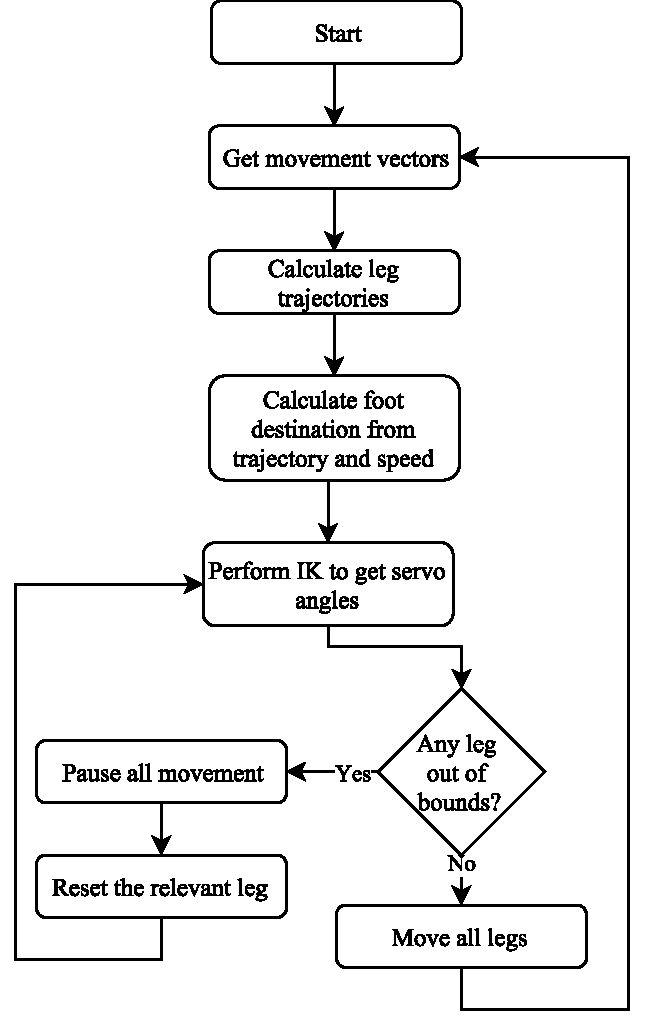
\includegraphics[scale = 1]{pics/Soft1.pdf}
\caption{Flow diagram showing robot walking algorithm.}
\label{fig:Soft1}
\end{figure}

While this is the core of the algorithm, some additional functions need to be included to make provision for some conditions. These are:
\begin{itemize}
\item Power is turned on initially.
\item Power is lost while in operation.
\item Power is regained.
\item Bluetooth is initially connected.
\item Bluetooth is suddenly disconnected.
\end{itemize}

A more complete diagram illustrating the design implemented on the microcontroller can be seen in Figure \ref{fig:Soft2}.\\

Servos are controlled with a square pulse with a specific width. The standard for hobbyist servo motors with a $180^o$ movement range is that a high pulse of $1ms$ equates to $0^o$ while $2ms$ results in $180^o$. The period of this signal is $20ms$.\\

A typical set of control signals for an analogue servo motor can be seen in figure \ref{fig:Servo1}.

\begin{figure}[H]
\centering
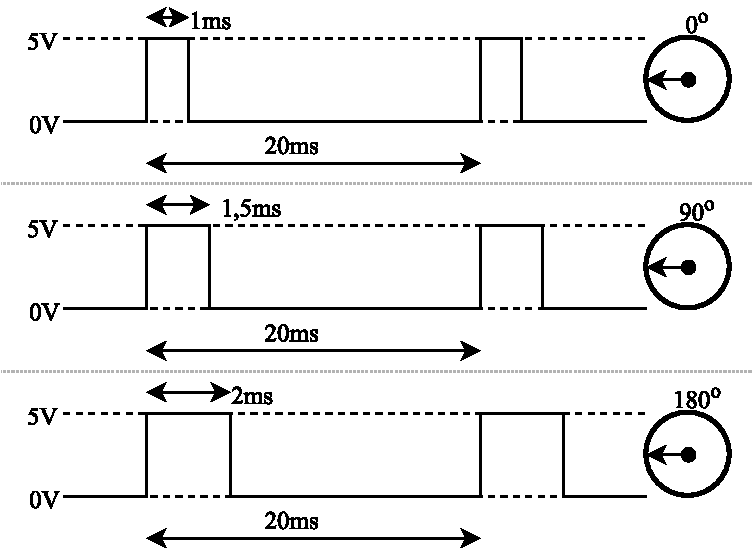
\includegraphics[scale = 1]{pics/Servo1.pdf}
\caption{Illustration of the working of a traditional servo control signal.}
\label{fig:Servo1}
\end{figure}

\begin{figure}[H]
\centering
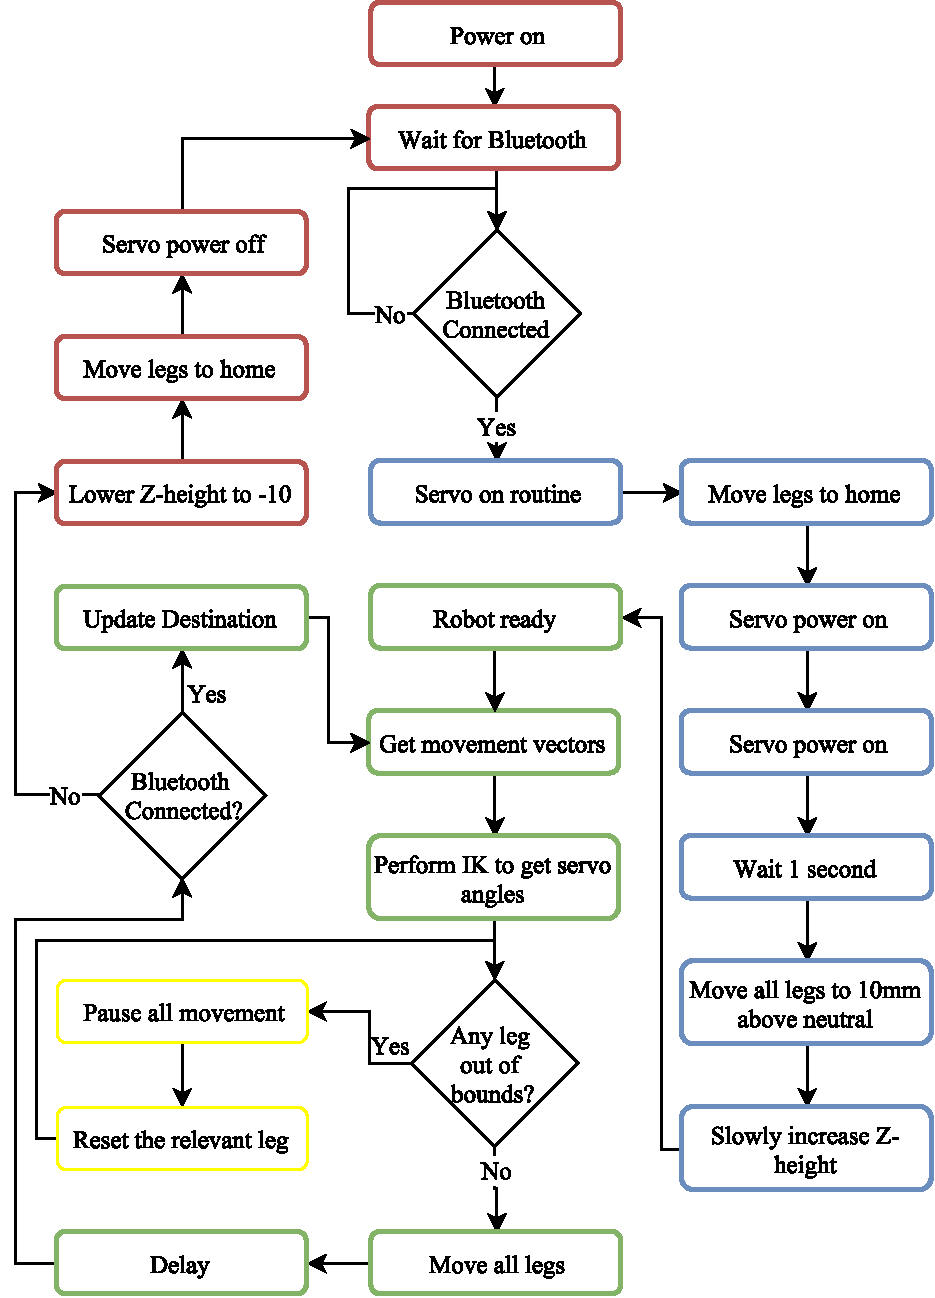
\includegraphics[scale = 1]{pics/Soft2.pdf}
\caption{Flow diagram showing robot walking algorithm final implementation.}
\label{fig:Soft2}
\end{figure}

In order to control the 15 servo motors on the robot simultaneously, 15 independent control signals like the ones shown in Figure \ref{fig:Servo1} should be generated. A common way to do this is to use the microcontroller's built-in pulse width modulation (PWM) module with a fixed frequency and variable duty cycle. While this is a valid approach for most cases, most microcontrollers don't have nearly enough independent PWM channels available to facilitate the 15 servo motors in this application.\\

Off-the-shelf modules that have a large number of PWM channels available and communicate with the microcontroller using the I2C, ISP or serial protocols are available but increases the electronic hardware components and power consumption.\\

The preferred solution in this case is using 15 normal digital output pins and two internal timers. One of the timers is set up to interrupt at $50Hz$, the period of the control signals. The second timer is reconfigured after each interrupt to have a new period. Figure \ref{fig:Servo2} attempts to illustrate how this procedure works for the simpler case of 5 servos.\\

\begin{table}[H]
\centering

\begin{tabular}{ccc}
\textbf{Servo} & \multicolumn{1}{l}{\textbf{Angle (deg)}} & \multicolumn{1}{l}{\textbf{Timer (ms)}} \\ \hline
1              & 45                                       & 1.25                                \\
2              & 90                                      & 1.5                                    \\
3              & 180                                      & 2                                       \\
4              & 0                                        & 1                                       \\
5              & 90                                      & 1.5                                    
\end{tabular}
\caption{Servo angles for the example explaining servo control using two timers.}
\label{tab:servo}
\end{table}

Before starting the procedure, Table \ref{tab:servo} is sorted in ascending order by the period in ms. The result can be seen in Table \ref{tab:servo2}

\begin{table}[H]
\centering

\begin{tabular}{cccc}
\textbf{Index} & \textbf{Servo} & \textbf{Angle (deg)} & \textbf{Timer (ms)} \\ \hline
1              & 4              & 0                    & 1                   \\
2              & 1              & 45                   & 1.25                \\
3              & 2              & 90                   & 1.5                 \\
4              & 5              & 90                   & 1.5                 \\
5              & 3              & 180                  & 2                  
\end{tabular}
\caption{Sorted servo angles for the example explaining servo control using two timers.}
\label{tab:servo2}
\end{table}

For the simplified case where 5 servo motors should be controlled, Table \ref{tab:servo} shows example values to illustrate the procedure. The procedure is outlined using the event letters shown in Figure \ref{fig:Servo2}.
\begin{enumerate}[label = \Alph*]
\item Timer 1 interrupts. All servo pins are set high. Timer 2 period is set to the timer value for index 1 (a=$1.25ms$).
\item Timer 2 interrupts. Servo for index 1 is set low (Servo 4). Timer 2 period is set to the timer value in index 2 - timer of index 1 (b=$1.25-1 = 0.25ms$).
\item Timer 2 interrupts. Servo for index 2 is set low (Servo 1). Timer 2 period is set to the timer value in index 3 - timer of index 2 (c=$1.5-1.25 = 0.25ms$).
\item Timer 2 interrupts. Servo for index 3 and 4 is set low (Servo 2 and 5). Timer 2 period is set to the timer value in index 5 - timer of index 4 (d=$2-1.5 = 0.5ms$).
\item Timer 2 interrupts. Servo for index 5 is set low (Servo 3). Timer 2 is turned off for the remainder of the $20ms$ ($e=NULL$)
\item Timer 1 interrupts. All servo pins are set high. Timer 2 period is set to the timer value for index 1 (a=$1.25ms$).
\item Timer 2 interrupts. Servo for index 1 is set low (Servo 4). Timer 2 period is set to the timer value in index 2 - timer of index 1 (b=$1.25-1 = 0.25ms$).
\item Timer 2 interrupts. Servo for index 2 is set low (Servo 1). Timer 2 period is set to the timer value in index 3 - timer of index 2 (c=$1.5-1.25 = 0.25ms$).
\item Timer 2 interrupts. Servo for index 3 and 4 is set low (Servo 2 and 5). Timer 2 period is set to the timer value in index 5 - timer of index 4 (d=$2-1.5 = 0.5ms$).
\item Timer 2 interrupts. Servo for index 5 is set low (Servo 3). Timer 2 is turned off for the remainder of the $20ms$ ($e=NULL$)
\end{enumerate}

\begin{figure}[H]
\centering
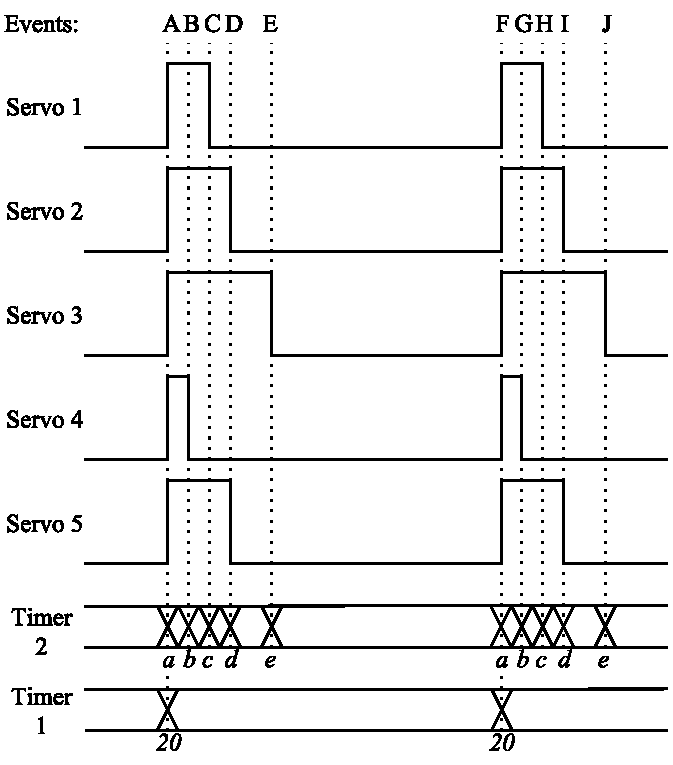
\includegraphics[scale = 1]{pics/Servo2.pdf}
\caption{Illustration of how multiple servo motors are controlled using two timers.}
\label{fig:Servo2}
\end{figure}

\subsubsection{Software implementation}
For the implementation of the program on the microcontroller, the C programming language together with the KEIL microcontroller development kit, which is an integrated development environment (IDE), was used. The STM32 series microcontrollers come with an application called CubeMX that can be used to generate initialization code for a specific microcontroller. This was used to configure all of the peripherals used as well as the system clock settings.\\

The algorithms developed and refined in Python was then translated to C and implemented in the software. Some of the functions implemented that were not included in the Python program are outlined below.\\


\begin{figure}[H]
\centering
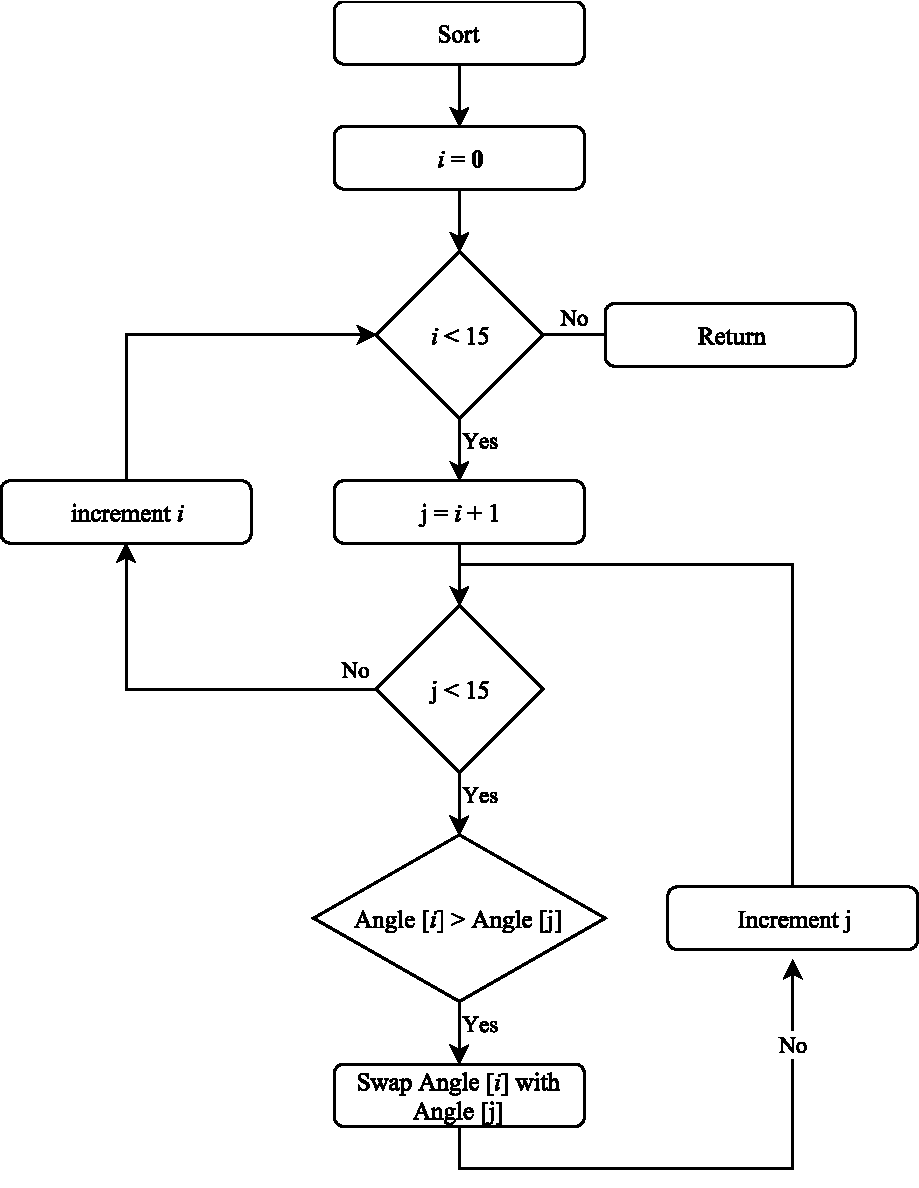
\includegraphics[scale = 1]{pics/Soft4.pdf}
\caption{Flow diagram showing the functioning of the sorting required by the servo algorithm.}
\label{fig:Soft4}
\end{figure}

Figure \ref{fig:Soft4} shows the functioning of the algorithm that sorts the servo times in ascending order. The sorting method used here is one of the simplest sorting methods, often referred to as bubble sorting. Since it is only 15 values being compared, it is not worth implementing a more complicated algorithm for the sake of efficiency\\

The timer interrupts are difficult to show in the main program flow because it is something that is constantly happening in the background. Figures \ref{fig:Soft5} through \ref{fig:Soft7} show the different timer interrupt service routines to show how this function works. It is important to not that timers 6 and 7 in Figure \ref{fig:Soft5} correspond to timers 1 and 2 respectively in Figure \ref{fig:Servo2} \\

\begin{figure}[H]
\centering
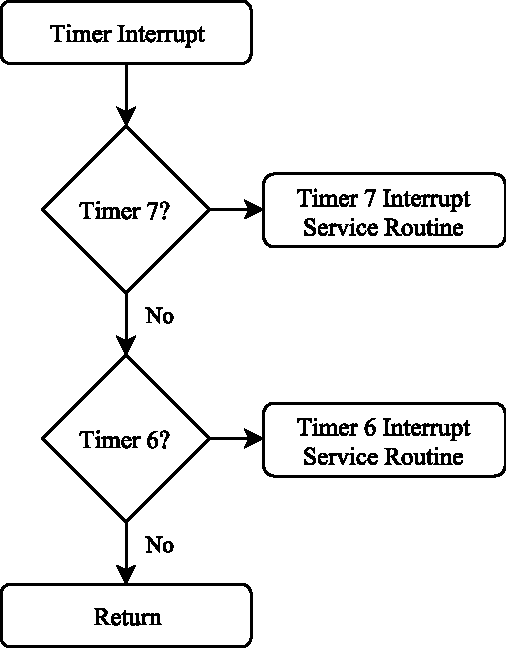
\includegraphics[scale = 1]{pics/Soft5.pdf}
\caption{Flow diagram showing the functioning of the main timer interrupt service routine.}
\label{fig:Soft5}
\end{figure}

\begin{figure}[H]
\centering
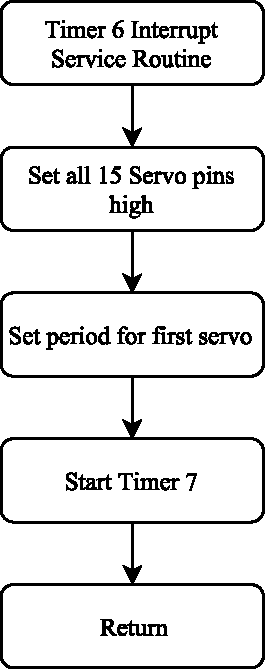
\includegraphics[scale = 1]{pics/Soft6.pdf}
\caption{Flow diagram showing the functioning of the timer 6 interrupt service routine.}
\label{fig:Soft6}
\end{figure}

\begin{figure}[H]
\centering
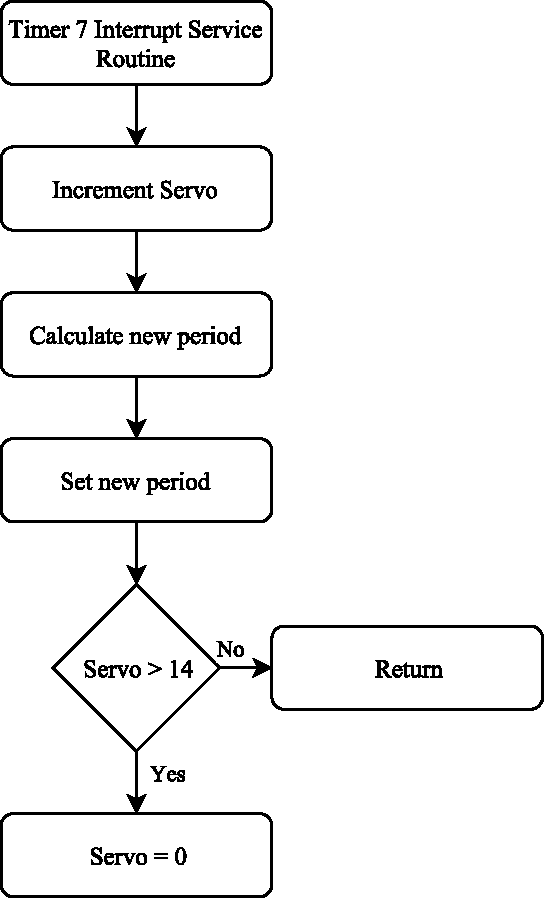
\includegraphics[scale = 1]{pics/Soft7.pdf}
\caption{Flow diagram showing the functioning of the timer 7 interrupt service routine.}
\label{fig:Soft7}
\end{figure}

The communication with the Bluetooth module makes use of the serial protocol. Once a message is received as a string. It should be checked for validity and then decoded to get usable integer values from this. The android application always sends data in the same format. Each of the values for X, Y and R is represented by a single integer digit. This value can't be negative since the minus sign would take up another character and everything would be out of alignment. The solution is to represent each number as a value between $-4$ and $4$, then add 5 to this number. The result is that a value of -4 would be represented by a $1$ and a value of $4$ represented by a $9$. They are then inserted in a mask of the following format: \textit{X\_Y\_R\_*} where the underscore is replaced by the appropriate character from $1$ to $9$ for each of the three values. If all of the values for X,Y and R are 0 from the UI, the resultant string would therefore be \textit{X5Y5R5*}. The decoding process is shown in Figure \ref{fig:Soft8}.\\

\begin{figure}[H]
\centering
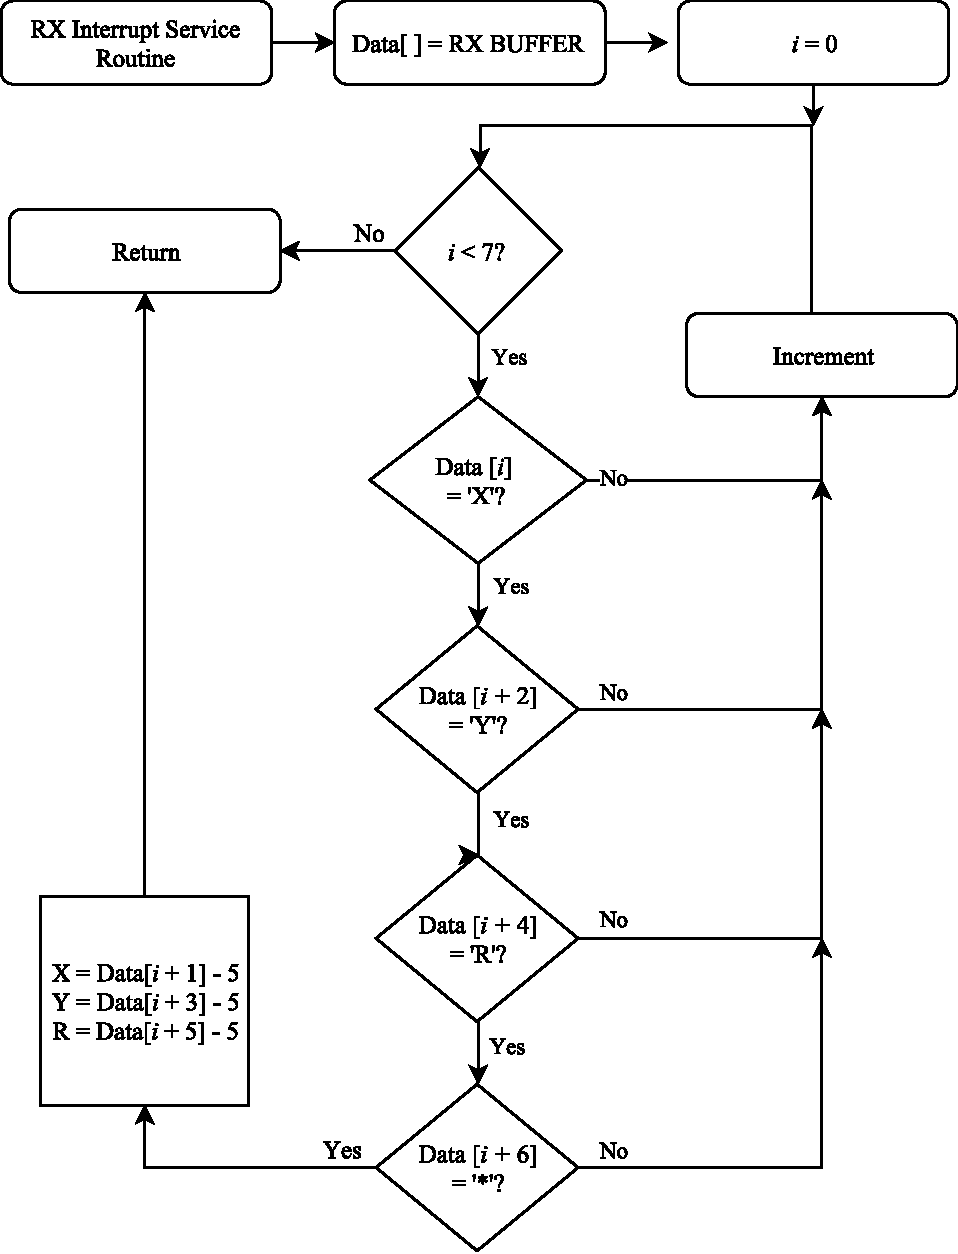
\includegraphics[scale = 1]{pics/Soft8.pdf}
\caption{Flow diagram showing the decoding of data from the Bluetooth module.}
\label{fig:Soft8}
\end{figure}
